\documentclass[notes=show]{beamer}
\usepackage{mathpazo}
\usepackage{hyperref}
\usepackage{multimedia}
\usepackage{tcolorbox}
\usepackage{tikz}
\usetikzlibrary{shadows}
\usetheme{metropolis}
\usecolortheme{default}
\setbeamertemplate{itemize item}{%
    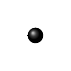
\begin{tikzpicture}
        \shade[ball color=black!100!yellow, preaction={fill=black,
opacity=.00,transform canvas={xshift=1mm,yshift=-1mm, yscale=0.5}}] (0,0) circle (0.6ex);
    \end{tikzpicture}
}
\setbeamertemplate{itemize subitem}{%
    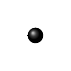
\begin{tikzpicture}
        \shade[ball color=black!100!white, preaction={fill=black,
        opacity=.00,transform canvas={xshift=1mm,yshift=-1mm, yscale=0.5}}] (0,0) circle (0.6ex);
    \end{tikzpicture}
}
\setbeamercolor{frametitle}{bg=white}
\setbeamercolor{frametitle}{fg=black}
\setbeamercolor{background canvas}{bg=white}
\setbeamercolor{block body}{bg=mDarkTeal!30}
\setbeamercolor{block title}{bg=mDarkTeal,fg=black!2}
\setbeamertemplate{navigation symbols}{}
\setbeamertemplate{footline}[page number]
\newenvironment{stepenumerate}{\begin{enumerate}[<+->]}{\end{enumerate}}
\newenvironment{stepitemize}{\begin{itemize}[<+->]}{\end{itemize} }
\newenvironment{stepenumeratewithalert}{\begin{enumerate}[<+-| alert@+>]}{\end{enumerate}}
\newenvironment{stepitemizewithalert}{\begin{itemize}[<+-| alert@+>]}{\end{itemize} }

\graphicspath{{figures/}}

\begin{document}

\title{Workplace Heterogeneity and the Rise of West German Wage Inequality}
\subtitle{}
\date{David Card, Jorg Heining, Patrick Kline \bigskip \\
\textit{Quarterly Journal of Economics}, August 2013}
\author{}
\maketitle

\AtBeginSection[ ]
{
\begin{frame}{Outline}
    \tableofcontents[currentsection]
\end{frame}
}

%%%%%%%%%%%%%%%%%%%%%%%%%%%%%%%%%%%%%%%%%%%%%%%%%%%%%%%%%%%%%%%%%
\section{Introduction}
%%%%%%%%%%%%%%%%%%%%%%%%%%%%%%%%%%%%%%%%%%%%%%%%%%%%%%%%%%%%%%%%%

\begin{frame}{Slichter (1950): a 1940 wage survey from Boston}
\begin{figure}[p!]
 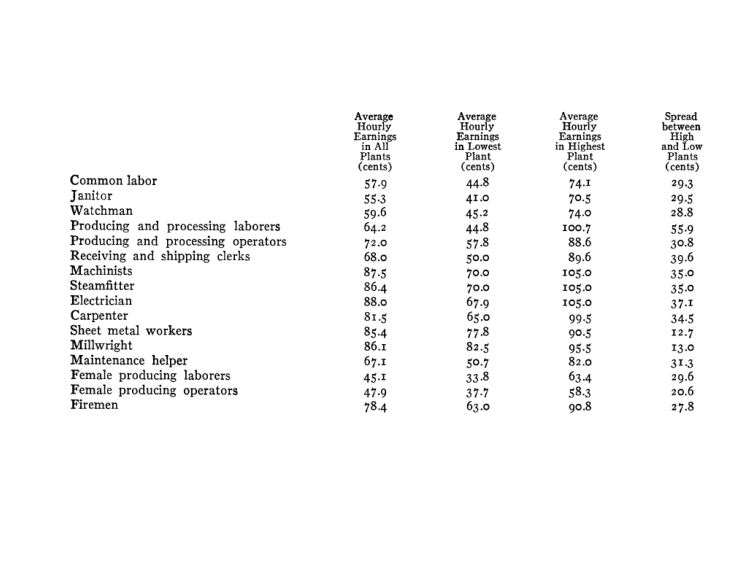
\includegraphics[width=\textwidth]{figures/Slichter.pdf} 
\end{figure}
\begin{center}
    ``\textit{Hourly earnings do not represent the price of labor.}''
\end{center}
\end{frame}

\begin{frame}{Slichter (1950): firms set wages}
\begin{enumerate}
    \item Positive correlation with wages of skilled co-workers
    \item Negative correlation with \% female
    \item Positive correlation with industry value-added/worker-hour
    \item Positive correlation with sales/worker-hour
    \item Negative correlation with payroll/sales
    \item Positive correlation with profit margin
    \item Stable over time (high correlation of industry wage rank)
\end{enumerate}
\begin{center}
    ``\textit{The results of this study give strong support to the proposition that managerial policy is important in firms setting wages.}''
\end{center}
\end{frame}

\begin{frame}{Krueger and Summers (1988): noncompetitive rents}
\begin{itemize}
    \item Was Slichter (1950) right that firms set wages? \medskip
    \item Use panel data and include worker FE to account for sorting between industries based on unmeasured ability. \medskip
    \item Industry wage-premia are similar to cross-sectional estimates. \medskip
    \item Industry wage-premia are not a compensating differential. \medskip
    \item People don't quit high wage jobs.
\end{itemize}
\begin{center}
    \textit{Workers in high-wage industries receive noncompetitive rents.}
\end{center}
\end{frame}

\begin{frame}{Variance of industry FE}
\begin{itemize}
    \item Target parameter is size weighted variance of industry effects:
    \begin{equation*}
        \theta_{\psi} \equiv Var(\psi_{j}) = \sum_{j=1}^{J} s_{j} (\psi_{j} - \bar{\psi})^2
    \end{equation*}
    where $s_{j}$ is firm $j$'s employment share and $\bar{\psi}=\sum_{j=1}^{J}s_{j}\psi_{j}$.
    \item Use OLS estimates $\hat{\psi_{j}}$ to compute ``plug-in'' estimates of variance components:
    \begin{align*}
         \hat{\theta}_{\psi} & = \sum_{j=1}^{J} s_{j} (\hat{\psi_{j}} - \hat{\bar{\psi}})^2 \\
         & = \sum_{j=1}^{J} s_{j} (\hat{\psi_{j}})^2 - (\hat{\bar{\psi}})^2
    \end{align*}
\end{itemize}
\end{frame}

\begin{frame}{Bias in the square of an unbiased estimate}
\begin{itemize}
    \item OLS estimates $ \hat{\psi_{j}} $ are unbiased:
    \begin{equation*}
        \mathbb{E} \left[ \hat{\psi_{j}} \right] = \psi_{j}
    \end{equation*}
    \item But the square of an unbiased estimator is upward biased:
    \begin{align*}
          \mathbb{E} \left[ \left( \hat{\psi_{j}} \right)^{2} \right] & =  \mathbb{E} \left[ \left( \hat{\psi_{j}} - \psi_{j} + \psi_{j} \right)^{2} \right] \\
          & = \mathbb{E} \left[ \left( \hat{\psi_{j}} - \psi_{j} \right) ^{2} \right] + 2 \mathbb{E} \left[ \hat{\psi_{j}} - \psi_{j} \right] \psi_{j} +  \psi_{j}^{2} \\
          & = \psi_{j}^{2} + \underbrace{ \mathbb{V} \left[ \hat{\psi_{j}} \right] }_{\text{bias}}
    \end{align*}
    \item Bias is the variance of estimated industry FE.
\end{itemize}
\end{frame}

\begin{frame}{Bias in plug-in estimator of variance of industry FE}
\begin{itemize}
    \item Similarly, the estimated variance of industry FE is biased:
    \begin{align*}
         \mathbb{E}  \left[ \hat{\theta}_{\psi} \right] & = \sum_{j=1}^{J} s_{j}  \mathbb{E}  \left[\hat{\psi_{j}}^2 \right] -  \mathbb{E}  \left[ \hat{\bar{\psi}}^2 \right] \\
         & = \sum_{j=1}^{J}s_{j} \left\{ \psi_{j}^{2} + \mathbb{V} \right[ \hat{\psi_{j}} \left] \right\} - \bar{\psi}^2 - \mathbb{V} \left[ \hat{\bar{\psi}}\right]
    \end{align*}
     \item When $J$ is large, the last term is negligible:
    \begin{equation*}
         \mathbb{E}  \left[ \hat{\theta}_{\psi} \right] \approx \theta_{\psi} + \underbrace{\sum_{j=1}^{J} s_{j} \mathbb{V} \left[ \hat{\psi_{j}} \right]}_{\text{bias}}
    \end{equation*}
    \item Bias is weighted variance of estimated industry FE.
\end{itemize}
\end{frame}

\begin{frame}{Substantial cross-sectional variability in industry wage-premia}
\begin{figure}[p!]
 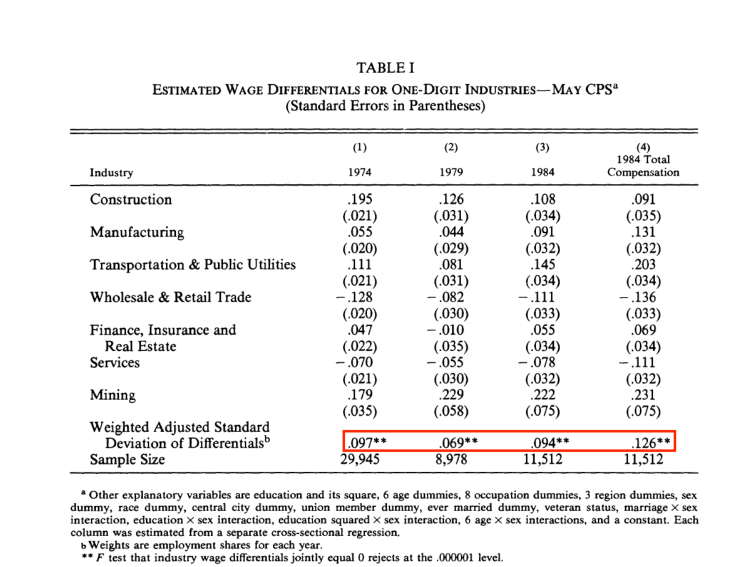
\includegraphics[width=0.9\textwidth]{CardHeiningKline/figures/KS-T1.pdf} 
\end{figure}
\end{frame}

\begin{frame}{Estimates including worker FE are similar}
\begin{figure}[p!]
 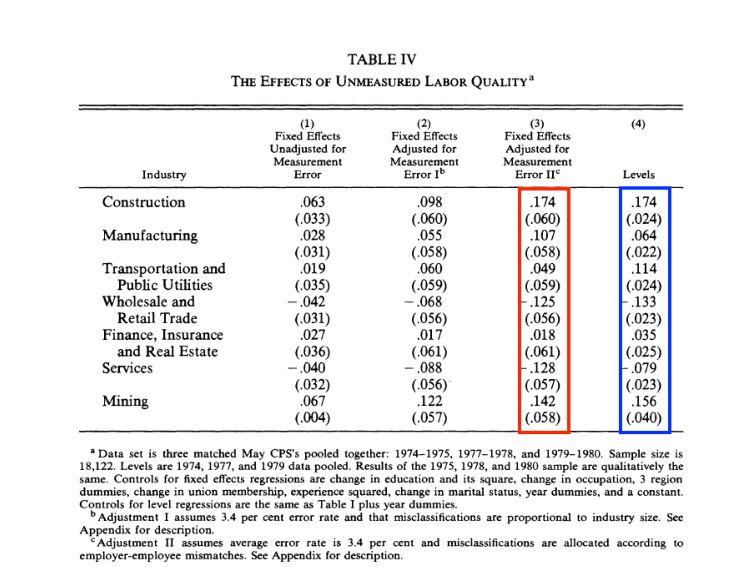
\includegraphics[width=.9\textwidth]{CardHeiningKline/figures/KS-T4.pdf} 
\end{figure}
\end{frame}

\begin{frame}{No evidence of compensating differentials}
\begin{figure}[p!]
 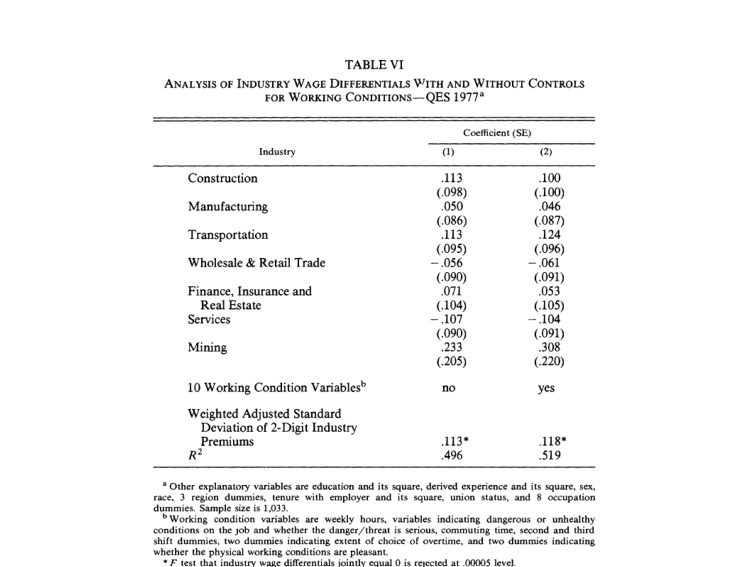
\includegraphics[width=.65\textwidth]{CardHeiningKline/figures/KS-T6.pdf} 
\end{figure}
\end{frame}

\begin{frame}{Workers don't quit high-wage jobs}
\begin{figure}[p!]
 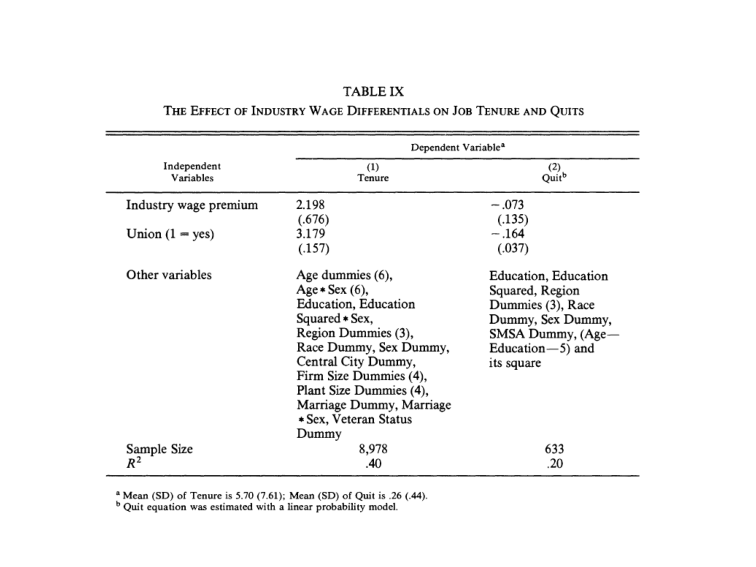
\includegraphics[width=.9\textwidth]{CardHeiningKline/figures/KS-T9.pdf} 
\end{figure}
\end{frame}

\begin{frame}{Abowd, Kramarz and Margolis (1999): AKM}
\begin{itemize}
    \item Use matched employer-employee data to study firm FE \medskip
    \item High-dimensional FE specification becomes:
    \begin{equation*}
        y_{it} = \alpha_i + \psi_{J(i,t)} + x'_{it}\beta + \epsilon_{it}
    \end{equation*}
    \item Key finding in constrast to Krueger and Summers (1988): 90\% of industry wage-premia attributable to person effects. \medskip
    \item However, can't invert design matrix with millions of FE. \medskip
    \item Instead, they use approximate solution method to estimate FE. 
\end{itemize}
\end{frame}

\begin{frame}{Revisiting Abowd, Kramarz and Margolis (1999)}
\begin{enumerate}
    \item \textbf{Abowd, Creecy and Kramarz (2002)}:
    \begin{itemize}
        \item Approximate FE very weakly correlated with exact FE in French data $ \Rightarrow$ original AKM results invalid! \smallskip
        \item Exact results find firm FE explain 55\% of variation in wages in France and 45\% in Washington state. \smallskip
        \item But $ Cov(\alpha_{i},\psi_{J(i,t)}) <0$ $\Rightarrow$ negative assortative matching?
    \end{itemize}
    \item \textbf{Abowd, Lengermann, and McKinney (2003)}:
    \begin{itemize}
        \item Use a 100\% sample extract from LEHD of 7 US states instead of small subsamples. \smallskip
        \item Firm FE explain 20\% of variation in wages (less inflation due to sampling error as we explained before). \smallskip
        \item Assortative matching becomes positive! (less limited-mobility bias because larger connected set as we'll discuss later)
    \end{itemize}
\end{enumerate}
\end{frame}

\begin{frame}{Card, Heining and Kline (2013): AKM revival}
\begin{itemize}
    \item Study changes in German wage structure. \medskip
    \item Earlier work by Dustmann, Ludsteck and Schoenberg (2009) documented increase in German wage dispersion. \medskip
    \item Interpreted within traditional SDI framework \medskip
    \item Typical view: S+D influence the price of skill, I is barrier to price adjustment. \medskip
    \item What about the importance of firms? \medskip
\end{itemize}
\end{frame}

%%%%%%%%%%%%%%%%%%%%%%%%%%%%%%%%%%%%%%%%%%%%%%%%%%%%%%%%%%%%%%%%%
\section{Data}
%%%%%%%%%%%%%%%%%%%%%%%%%%%%%%%%%%%%%%%%%%%%%%%%%%%%%%%%%%%%%%%%%

%%%%%%%%%%%%%%%%%%%%%%%%%%%%%%%%%%%%
\subsection*{Data}
%%%%%%%%%%%%%%%%%%%%%%%%%%%%%%%%%%%%

\begin{frame}
	\centering
	\textbf{Data}
\end{frame}

\begin{frame}
\begin{figure}[p!]
	\begin{adjustbox}
        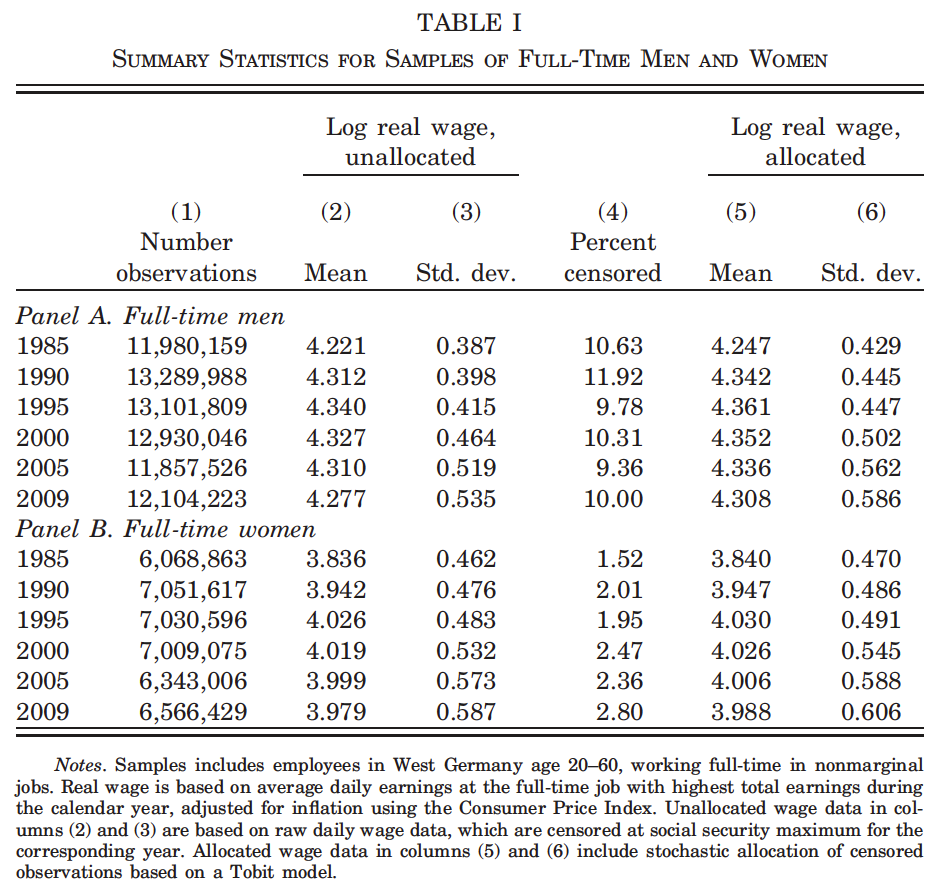
\includegraphics[width=.85\textwidth]{figures/Table1} 
 	\end{adjustbox}
\end{figure}
\end{frame}

%%%%%%%%%%%%%%%%%%%%%%%%%%%%%%%%%%%%
\subsection*{Trends in Wage Inequality}
%%%%%%%%%%%%%%%%%%%%%%%%%%%%%%%%%%%%

\begin{frame}
	\centering
	\textbf{Trends in Wage Inequality}
\end{frame}

\begin{frame}{Rise in wage inequality}
\begin{figure}[p!]
 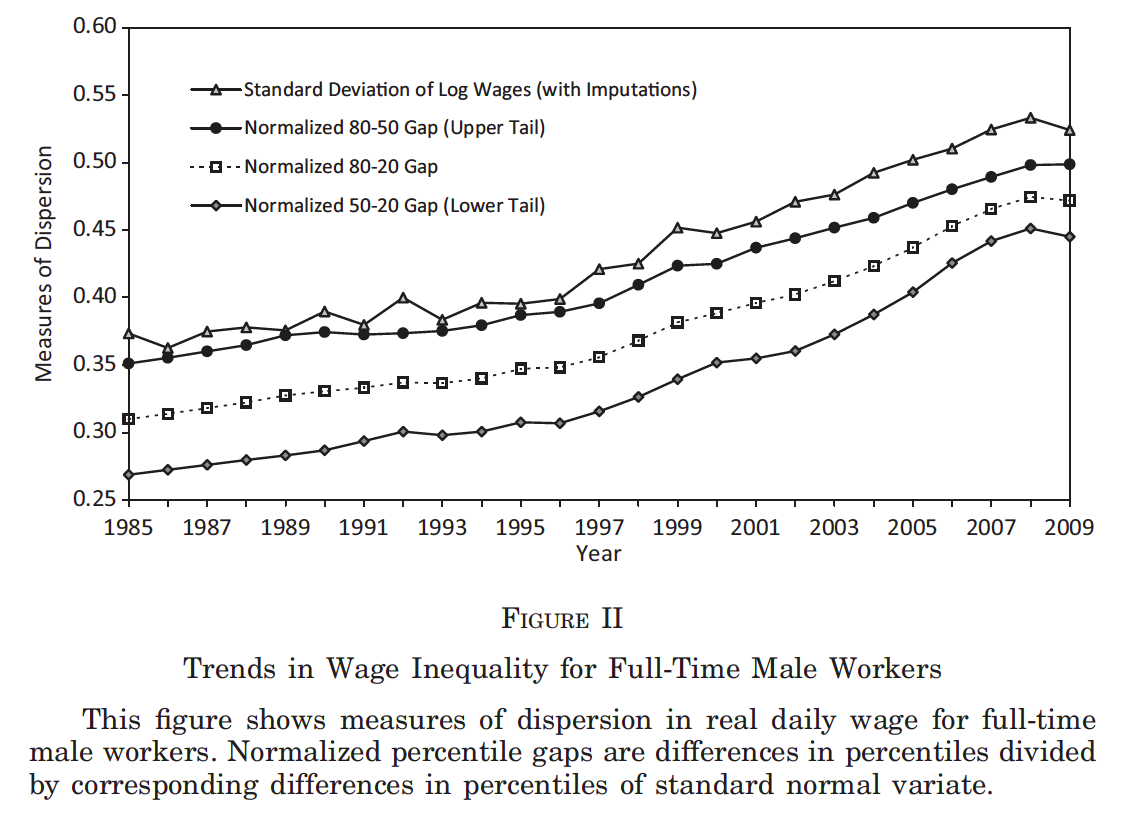
\includegraphics[width=.9\textwidth]{figures/Fig2} 
\end{figure}
\end{frame}

\begin{frame}{Overlapping intervals}
\begin{figure}[p!]
 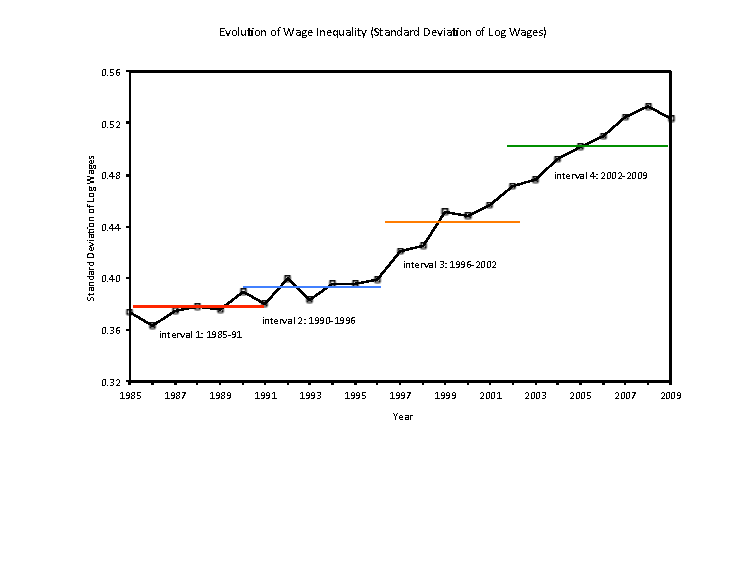
\includegraphics[width=\textwidth]{CardHeiningKline/figures/slide365.pdf} 
\end{figure}
\end{frame}

\begin{frame}{Focus on full-time jobs held by men between age 20-60}
\begin{figure}[p!]
 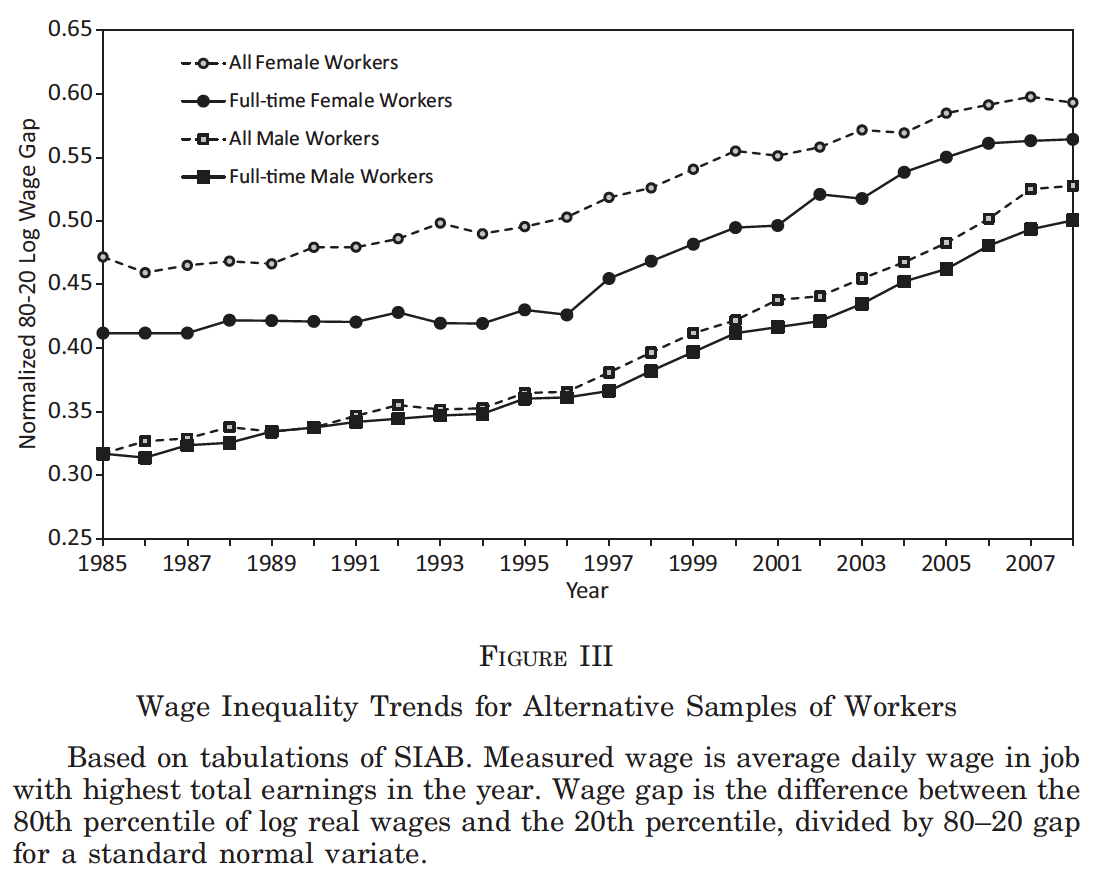
\includegraphics[width=.9\textwidth]{figures/Fig3} 
\end{figure}
\end{frame}

\begin{frame}{Growth in wage inequality primarily between firms}
\begin{figure}[p!]
 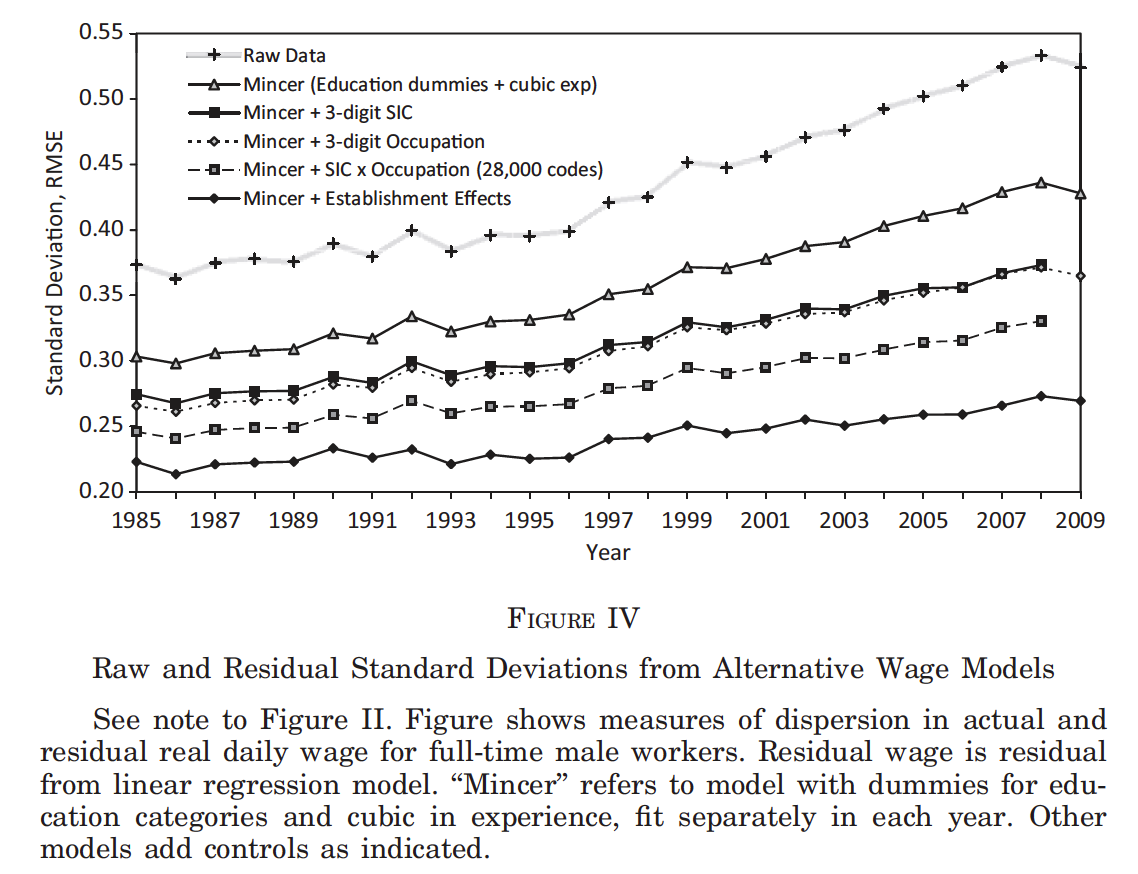
\includegraphics[width=.9\textwidth]{figures/Fig4} 
\end{figure}
\end{frame}

%%%%%%%%%%%%%%%%%%%%%%%%%%%%%%%%%%%%
\subsection*{Effect of Job Changes on Wages}
%%%%%%%%%%%%%%%%%%%%%%%%%%%%%%%%%%%%

\begin{frame}
	\centering
	\textbf{Effect of Job Changes on Wages}
\end{frame}

\begin{frame}{Effect of Job Changes on Wages}
	\begin{itemize}
		\item If wage variation across firms is due to workers sorting based on unobserved ability, then workers changing firms do not experience systematic changes in wages. \medskip
		\item But if different firms pay different wage premia to all their workers, then workers who join high-wage (low-wage) firms  experience a wage gain (loss). \medskip 
		\item Examine effect of moving to another firm on individual wages between 1985-1991 and 2002-2009. \medskip
		\item Origin workplace and destination workplace defined by average coworker wages.
	\end{itemize}
\end{frame}

\begin{frame}{Wage dynamics of job changes}
\begin{figure}[p!]
 \includegraphics[width=.65\textwidth]{CardHeiningKline/figures/Fig5.png} 
\end{figure}
\end{frame}

%%%%%%%%%%%%%%%%%%%%%%%%%%%%%%%%%%%%%%%%%%%%%%%%%%%%%%%%%%%%%%%%%
\section{Econometric Model}
%%%%%%%%%%%%%%%%%%%%%%%%%%%%%%%%%%%%%%%%%%%%%%%%%%%%%%%%%%%%%%%%%

\begin{frame}{AKM estimator}
%Data set contains N* person-year observations on N workers and J establishments \\
\begin{itemize} 
    \item Log daily real wage $y_{it}$ of individual $i$ in year $t$ is given by:
    \begin{equation} \label{eq_AKM}
	y_{it} = \alpha_i + \psi_{J(i,t)} + x'_{it}\beta + r_{it}
    \end{equation}
\item In matrix notation:
\begin{equation}
    y = D \alpha + F \psi + X \beta +r = Z' \xi + r
\end{equation}
\item OLS solves the standard normal equations:
\begin{equation}
    Z'Z \xi = Z'y
\end{equation}
\item Use matlab packages to find the ``largest connected set'' and solve normal equations using preconditioned conjugate gradient routine.
\end{itemize}
\end{frame}

\begin{frame}{Largest connected set}
\begin{figure}[p!]
 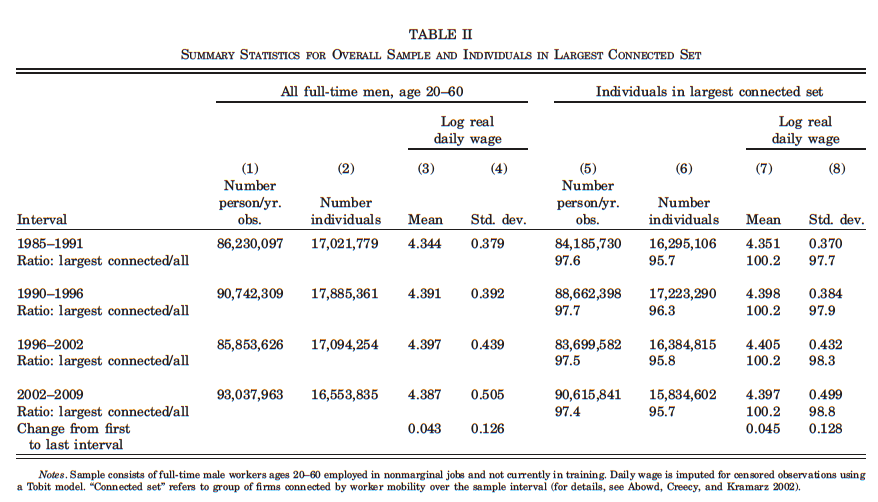
\includegraphics[width=\textwidth]{figures/Table2} 
\end{figure}
\end{frame}

\begin{frame}{Exogeneity assumptions}
\begin{itemize}
\item OLS requires the following independence conditions to hold:
\begin{equation} \label{eq_exogeneity}
	\forall i: E[d^{i}{'}r]=0 ; \forall j: E[f^{j}{'}r]=0 ; \forall k: E[x^{k}{'}r]=0 
\end{equation}
\item $\forall k: E[x^{k}{'}r]=0$ is standard assumption that error term is independent of time-varying covariates. \medskip
\item $\forall i: E[d^{i}{'}r]=0$ holds if all components of the error term have mean zero for each worker across years. \medskip
\item $\forall j: E[f^{j}{'}r]=0$ assumes that there is no sorting of workers to firms based on time-varying unobserved components of wages.
%Composite error term orthogonal to vector of establishment identifiers
\end{itemize}
\end{frame}

\begin{frame}{Specifying the error term}
\begin{itemize}
\item Assume $r_{it}$ consists of three separate random effects:
\begin{equation*}
	r_{it} = \eta_{iJ(i,t)} + \zeta_{it} + \epsilon_{it}
\end{equation*}
with
\begin{itemize}
    \item $\eta_{iJ(i,t)}$ an idiosyncratic match component \smallskip
    \item $\zeta_{it}$ drift in a portable component \smallskip
    \item $\epsilon_{it}$ a mean-reversing transitory component. \smallskip
\end{itemize}
\item We assume that $\forall k: E[x^{k}{'}r]=0$ and $\forall i: E[d^{i}{'}r]=0$. \medskip
\item Condition $\forall j: E[f^{j}{'}r]=0$ requires that sorting of workers to firms based on time-varying unobserved component of wages is independent of firm FE.
\end{itemize}
\end{frame}

\begin{frame}{Exogenous assignment of workers to firms}
\begin{itemize}
    \item Sufficient condition is that assignment of workers to firms is independent of $r$:
    \begin{equation}
	P(J(i,t)=j|r)=P(J(i,t)=j)=G_{jt}(\alpha_i, \psi_1,...,\psi_J) 
    \end{equation}
with $G_{jt}$ the employment probability function summing to 1 for every worker in every period. \medskip
    \item Systematic patterns of job mobility based on unobserved person-effects and firm-effects allowed! \medskip
    \item The paper discusses 3 violations.
\end{itemize}
\end{frame}

\begin{frame}{V1: Selection on match component ($Cov(\psi_{j},\eta_{ij}) \neq 0$)}
	\begin{itemize}
		\item Possible if lots of scope for comparative advantage (a la Roy (1952)) and worker has bargaining power. \medskip
            \item Transitions in both directions should usually be associated with wage increases:
            \begin{align*}
                \mathbb{E} \left[ y_{i,t} - y_{i,t-1} | 1 \rightarrow 4 \right] & = - \psi_{1} + \psi_{4} + \mathbb{E} \left[ \eta_{i,4} - \eta_{i,1} | 1 \rightarrow 4 \right] \\
                \mathbb{E} \left[ y_{i,t} - y_{i,t-1} | 4 \rightarrow 1 \right] & = \psi_{1} - \psi_{4} + \mathbb{E} \left[ \eta_{i,1} - \eta_{i,4} | 4 \rightarrow 1 \right]
            \end{align*}
            \item And unrestricted match effects model should fit much better than worker FE + firm FE.
	\end{itemize}
\end{frame}

\begin{frame}
\begin{figure}[p!]
	\begin{adjustbox}
 \includegraphics[width=.75\textwidth]{figures/Fig5} 
 	\end{adjustbox}
\end{figure}
\end{frame}

\begin{frame}{V2: Selection on drift component ($Cov(\psi_{j},\zeta_{it}) \neq 0$)}
	\begin{enumerate}
		\item Possible if firms learn rapidly about workers and learning is associated with job-to-job mobility (Gibbons \& Katz, 1992). \medskip
            \item But, learning takes years (Lange, 2007). 
            \begin{itemize} \smallskip
                \item[-] Ought to see an increasing trend in event study before upward transitions and decreasing trend before downward transitions.
            \end{itemize} \medskip
            \item Another violation would be offer shopping in job ladder models (e.g. Postel‐Vinay and Robin, 2002)
            \begin{itemize} \smallskip
                \item[-] Difficulty explaining symmetry in event study. 
            \end{itemize}
	\end{enumerate}
\end{frame}

\begin{frame}
\begin{figure}[p!]
	\begin{adjustbox}
 \includegraphics[width=.75\textwidth]{figures/Fig5} 
 	\end{adjustbox}
\end{figure}
\end{frame}

\begin{frame}{V3: Selection on transitory component ($Cov(\psi_{j},\epsilon_{it}) \neq 0$)}
	\begin{itemize}
	\item Possible if firm has a bad year, wages fall, and people leave the following year. \medskip
        \item Understate the establishment effect at origin and overstates it at destination. \medskip
        \item But should see an Ashenfelter (1978) style dip in event study. \medskip
        \item Also: shocks at each firm should eventually average out to zero as T grows large.
	\end{itemize}
\end{frame}

\begin{frame}
\begin{figure}[p!]
	\begin{adjustbox}
 \includegraphics[width=.75\textwidth]{figures/Fig5} 
 	\end{adjustbox}
\end{figure}
\end{frame}

%%%%%%%%%%%%%%%%%%%%%%%%%%%%%%%%%%%%%%%%%%%%%%%%%%%%%%%%%%%%%%%%%
\section{Results}
%%%%%%%%%%%%%%%%%%%%%%%%%%%%%%%%%%%%%%%%%%%%%%%%%%%%%%%%%%%%%%%%%

%%%%%%%%%%%%%%%%%%%%%%%%%%%%%%%%%%%%
\subsection*{AKM Results}
%%%%%%%%%%%%%%%%%%%%%%%%%%%%%%%%%%%%

\begin{frame}
	\centering
	\textbf{AKM Results}
\end{frame}

\begin{frame}{Wage dynamics of job changes with firm FE}
\begin{figure}[p!]
 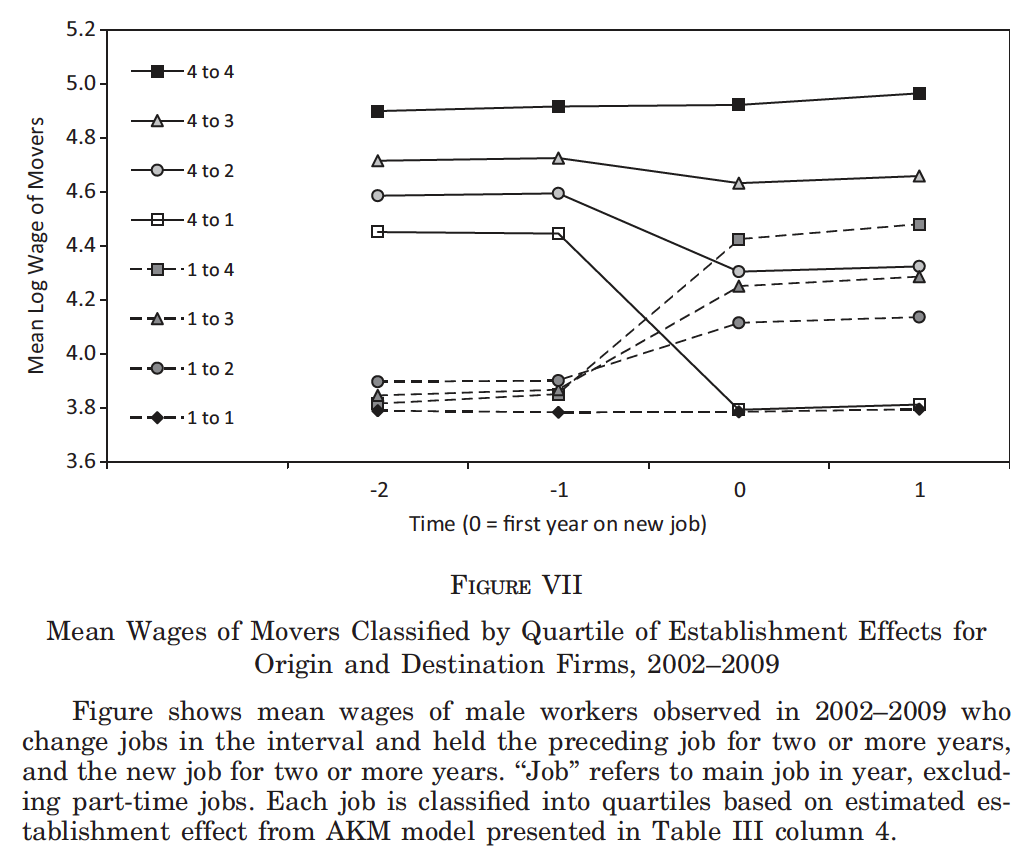
\includegraphics[width=.9\textwidth]{figures/Fig7.png} 
\end{figure}
\end{frame}

\begin{frame}{AKM estimates}
\begin{figure}[p!]
 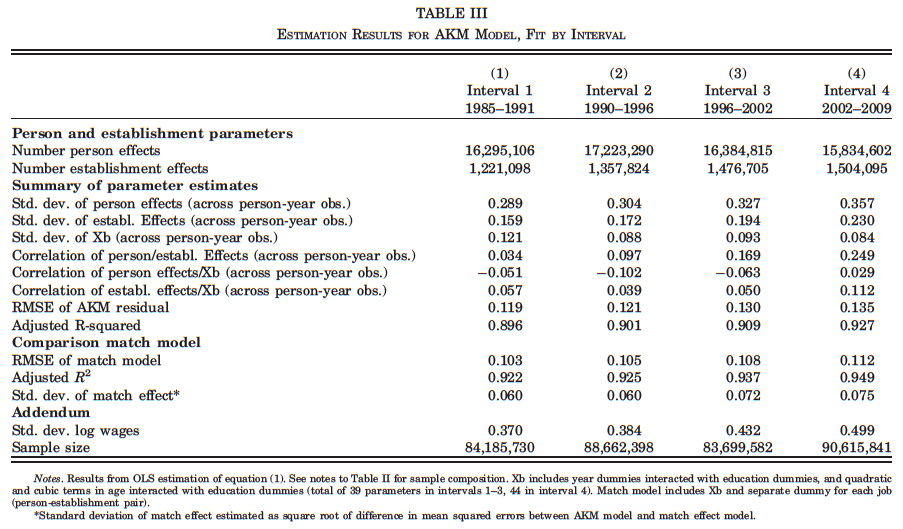
\includegraphics[width=\textwidth]{figures/Table3} 
\end{figure}
\end{frame}

\begin{frame}{Standard deviation of worker FE effects has increased}
\begin{figure}[p!]
 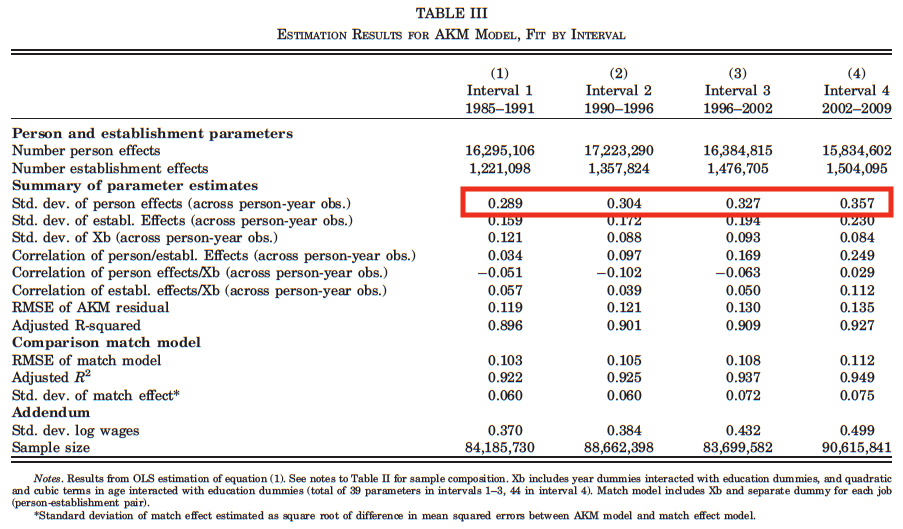
\includegraphics[width=\textwidth]{figures/Table3b} 
\end{figure}
\end{frame}

\begin{frame}{Standard deviation of firm FE has increased}
\begin{figure}[p!]
 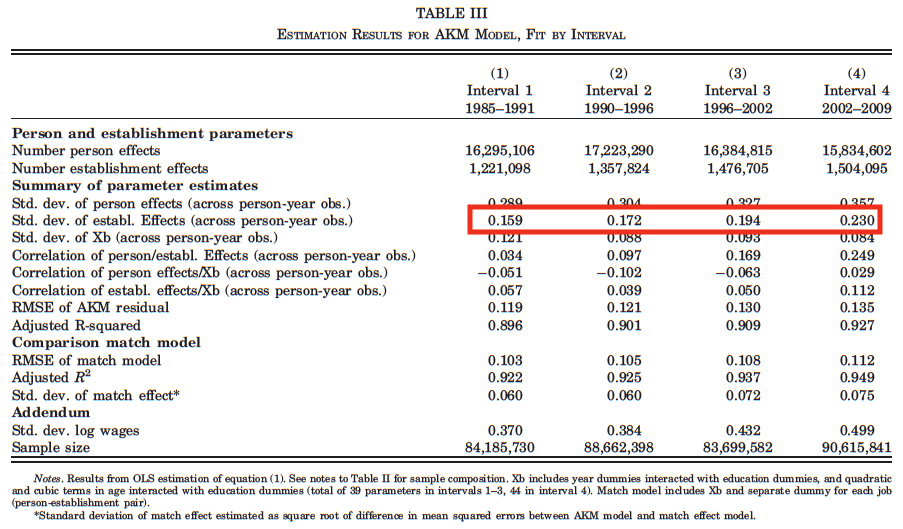
\includegraphics[width=\textwidth]{figures/Table3c} 
\end{figure}
\end{frame}

\begin{frame}{Positive assortative matching has increased}
\begin{figure}[p!]
 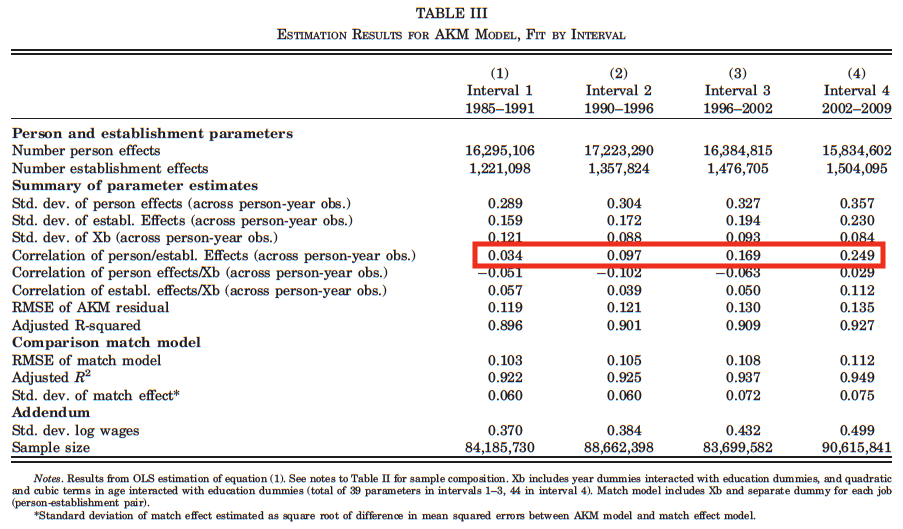
\includegraphics[width=\textwidth]{figures/Table3d} 
\end{figure}
\end{frame}

\begin{frame}{Positive assortative matching has increased}
\begin{figure}[p!]
	\begin{adjustbox}
 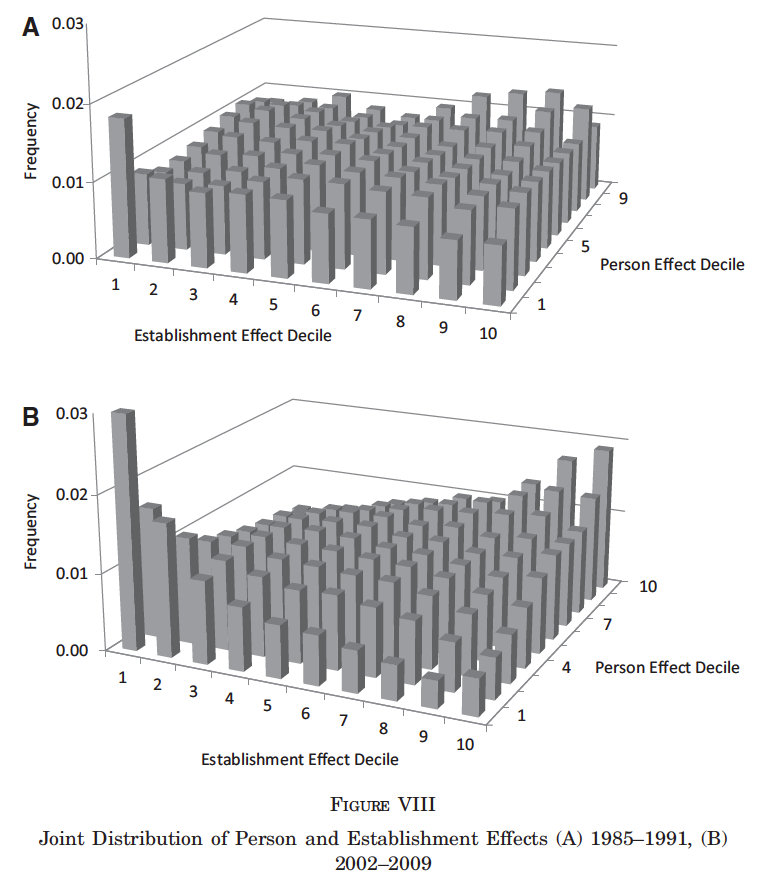
\includegraphics[width=.65\textwidth]{figures/Fig8}
 	\end{adjustbox} 
\end{figure}
\end{frame}

%%%%%%%%%%%%%%%%%%%%%%%%%%%%%%%%%%%%
\subsection*{Variance decomposition}
%%%%%%%%%%%%%%%%%%%%%%%%%%%%%%%%%%%%

\begin{frame}
	\centering
	\textbf{Variance decomposition}
\end{frame}

\begin{frame}{Variance decomposition}
\begin{itemize}
    \item Variance of wages can be decomposed as:
	\begin{equation}
	\begin{split}
		Var(y_{it})& = Var(\alpha_i)+Var(\psi_{J(i,t)})+Var(x_{it}'\beta) \\
				&+ 2Cov(\alpha_i,\psi_{J(i,t)})+2Cov(\psi_{J(i,t)},x_{it}'\beta) \\
				&+ 2Cov(\alpha_i,x_{it}'\beta) + Var(r_{it})
	\end{split}
	\end{equation}
 \item $ Var(\hat{\alpha}_{i}) $ and $ Var(\hat{\psi}_{J(i,t)}) $ are upward biased \medskip
 \item $Cov(\hat{\alpha}_i, \hat{\psi}_{J(i,t)}) $ are downward biased due to limited-mobility bias in small largest connected sets (Andrews et al. 2008) \medskip
 \item No bias corrections assuming no trend in biases over intervals
\end{itemize}
\end{frame}

\begin{frame}
\begin{figure}[p!]
 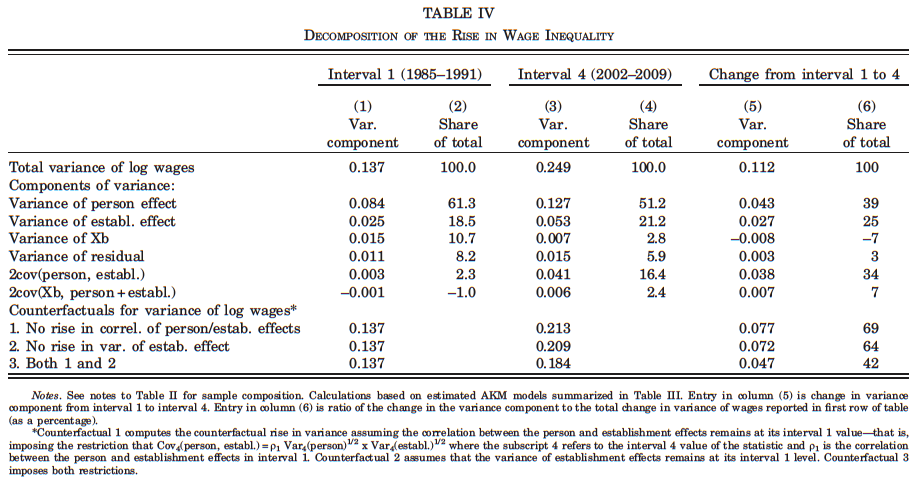
\includegraphics[width=\textwidth]{figures/Table4} 
\end{figure}
\end{frame}

\begin{frame}
\begin{figure}[p!]
 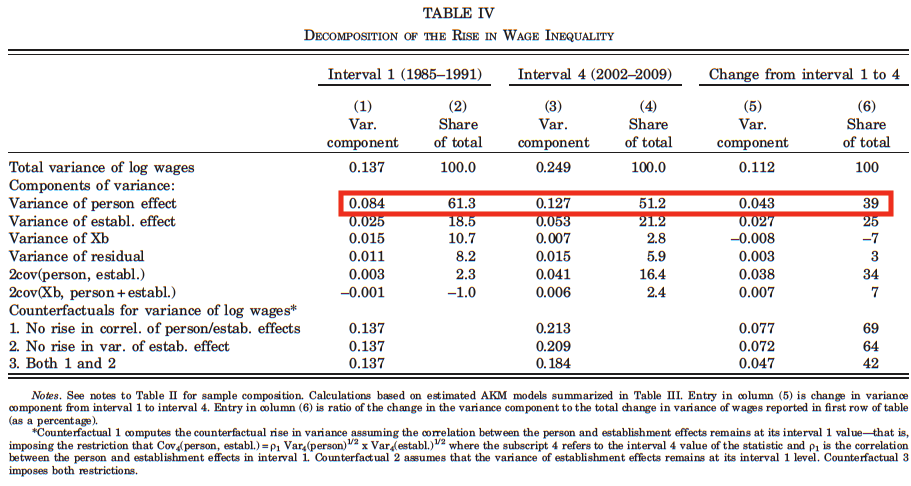
\includegraphics[width=\textwidth]{figures/Table4b} 
\end{figure}
\end{frame}

\begin{frame}
\begin{figure}[p!]
 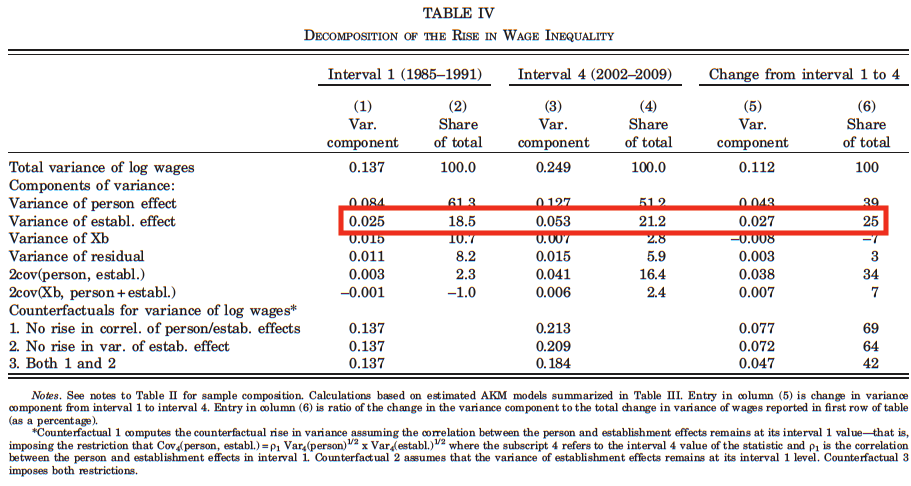
\includegraphics[width=\textwidth]{figures/Table4c} 
\end{figure}
\end{frame}

\begin{frame}
\begin{figure}[p!]
 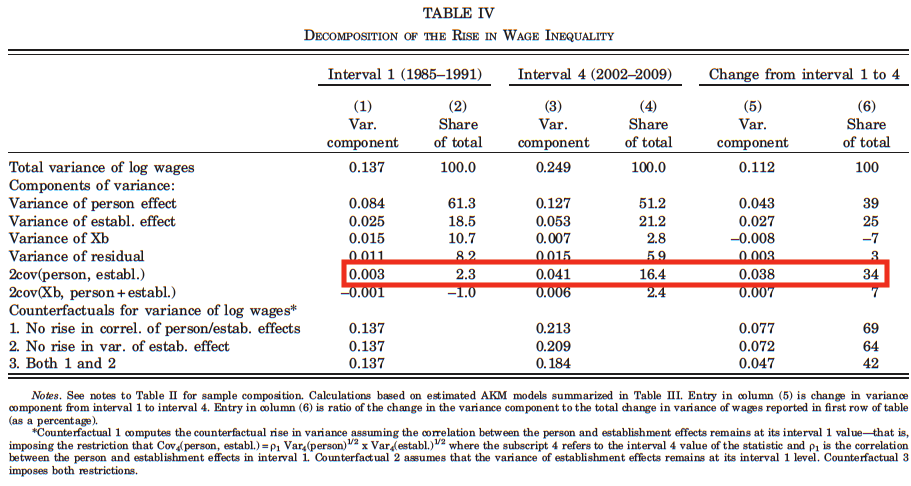
\includegraphics[width=\textwidth]{figures/Table4d} 
\end{figure}
\end{frame}

\begin{frame}{Rising variance of FE and sorting in rising variance of wages}
\begin{figure}[p!]
 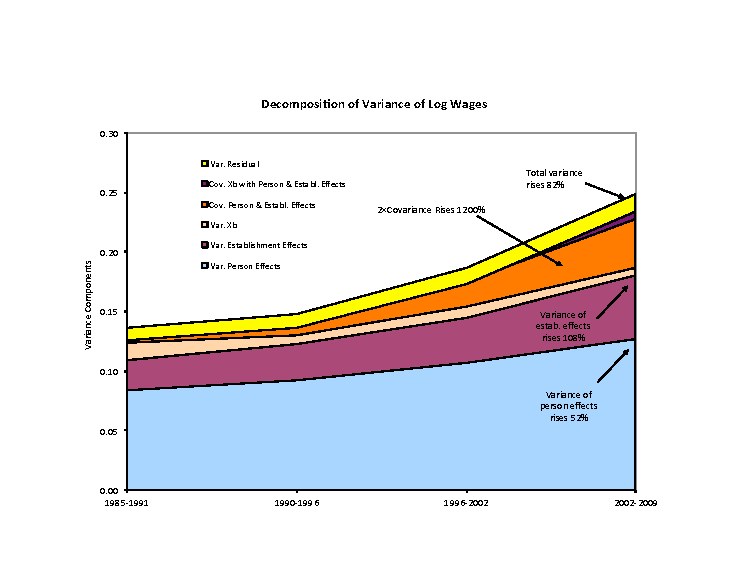
\includegraphics[width=\textwidth]{CardHeiningKline/figures/slide373.pdf} 
\end{figure}
\end{frame}

%%%%%%%%%%%%%%%%%%%%%%%%%%%%%%%%%%%%%%%%%%%%%%%%%%%%%%%%%%%%%%%%%
\section{Decomposing between-group wage differentials}
%%%%%%%%%%%%%%%%%%%%%%%%%%%%%%%%%%%%%%%%%%%%%%%%%%%%%%%%%%%%%%%%%

%%%%%%%%%%%%%%%%%%%%%%%%%%%%%%%%%%%%
\subsection*{Education}
%%%%%%%%%%%%%%%%%%%%%%%%%%%%%%%%%%%%

\begin{frame}
	\centering
	\textbf{Education}
\end{frame}

\begin{frame}{Comparing changes over time in group averages}
\begin{itemize}
\item From (\ref{eq_AKM}) and (\ref{eq_exogeneity}), the mean wage for workers in group $g$ is:
    \begin{equation} \label{eq_group_means}
	   \mathbb{E}_{g} \left[ y_{it} \right] = \mathbb{E}_{g} \left[ \alpha_{i} \right] + \mathbb{E}_{g} \left[ \psi_{J(i,t)} \right] + \mathbb{E}_{g} \left[ x_{it}'\beta \right]
    \end{equation}
    where $ \mathbb{E}_{g} \left[ . \right] \equiv \mathbb{E} \left[ . | G_{i}=g \right]$. \medskip
\item The change over time in the mean wage differential between groups $g_{1}$ and $g_{2}$ is given by:
    \begin{equation*}
	  \left\{ \mathbb{E}_{g_{1}} \left[ y_{i,t} \right] - \mathbb{E}_{g_{1}} \left[ y_{i,t-1} \right] \right\} -  \left\{ \mathbb{E}_{g_{2}} \left[ y_{i,t} \right] - \mathbb{E}_{g_{2}} \left[ y_{i,t-1} \right] \right\}
    \end{equation*}
 \end{itemize}
\end{frame}

\begin{frame}{Increasing return to schooling due to firm FE and sorting}
\begin{figure}[p!]
 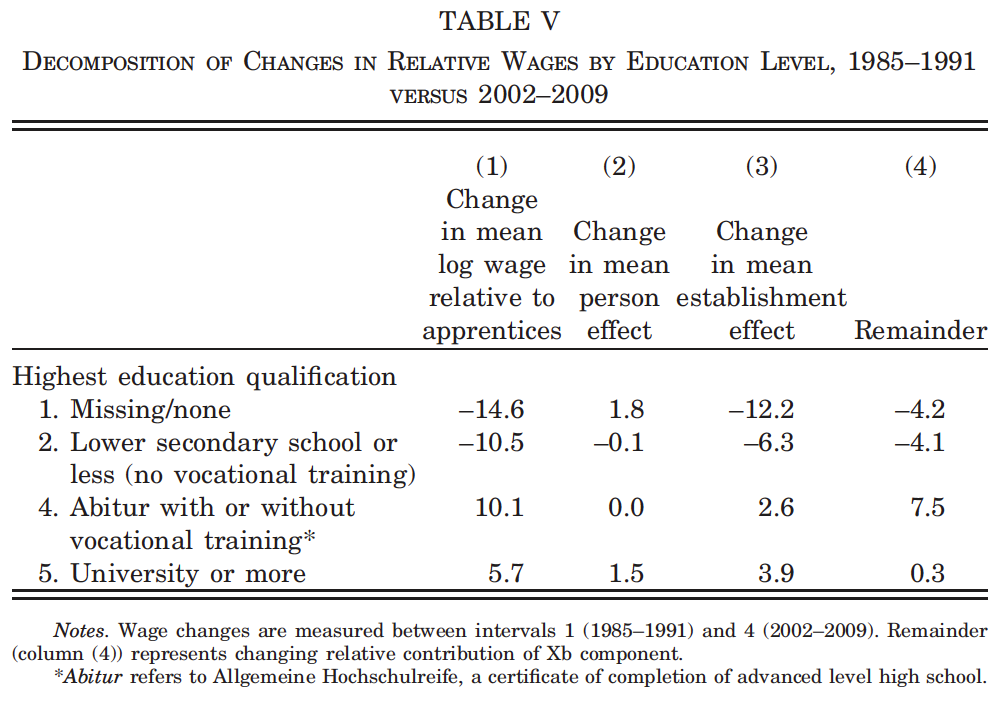
\includegraphics[width=\textwidth]{figures/Table5} 
\end{figure}
\end{frame}

%%%%%%%%%%%%%%%%%%%%%%%%%%%%%%%%%%%%
\subsection*{Occupation and Industry}
%%%%%%%%%%%%%%%%%%%%%%%%%%%%%%%%%%%%

\begin{frame}
	\centering
	\textbf{Occupation and Industry}
\end{frame}

\begin{frame}{Decomposing the variance of group averages}
\begin{itemize}
\item From (\ref{eq_group_means}), the variance in mean wages across groups is:
    \begin{align}
	   Var(\mathbb{E}_{g} \left[ y_{it} \right]) & = Var(\mathbb{E}_{g} \left[ \alpha_{i} \right]) \\
    & + Var(\mathbb{E}_{g} \left[ \psi_{J(i,t)} \right]) \nonumber \\
    & + Var(\mathbb{E}_{g} \left[ x_{it}'\beta \right]) \nonumber \\
    & + 2 Cov(\mathbb{E}_{g} \left[ \alpha_{i} \right]),\mathbb{E}_{g} \left[ \psi_{J(i,t)} \right]) \nonumber \\
    &  + 2 Cov(\mathbb{E}_{g} \left[ \alpha_{i} \right]),\mathbb{E}_{g} \left[ x_{it}'\beta \right]) \nonumber \\
    & + 2 Cov(\mathbb{E}_{g} \left[ \psi_{J(i,t)} \right],\mathbb{E}_{g} \left[ x_{it}'\beta \right]) \nonumber
    \end{align}
\item For $g$ occupation or industry, compare this decomposition in different time intervals.
 \end{itemize}
\end{frame}

\begin{frame}{Firms and sorting important in changing variance of premia}
\begin{figure}
 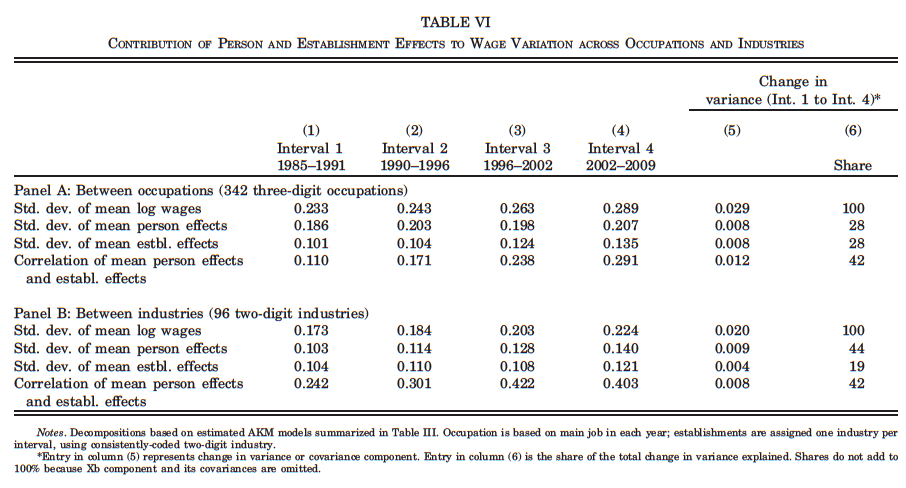
\includegraphics[width=\textwidth]{figures/Table6} 
\end{figure}
\end{frame}

%%%%%%%%%%%%%%%%%%%%%%%%%%%%%%%%%%%%%%%%%%%%%%%%%%%%%%%%%%%%%%%%%
\section{Institutional change as explanation}
%%%%%%%%%%%%%%%%%%%%%%%%%%%%%%%%%%%%%%%%%%%%%%%%%%%%%%%%%%%%%%%%%

\begin{frame}{Std. dev. of firm FE increased due to de-unionisation}
\begin{figure}[p!]
 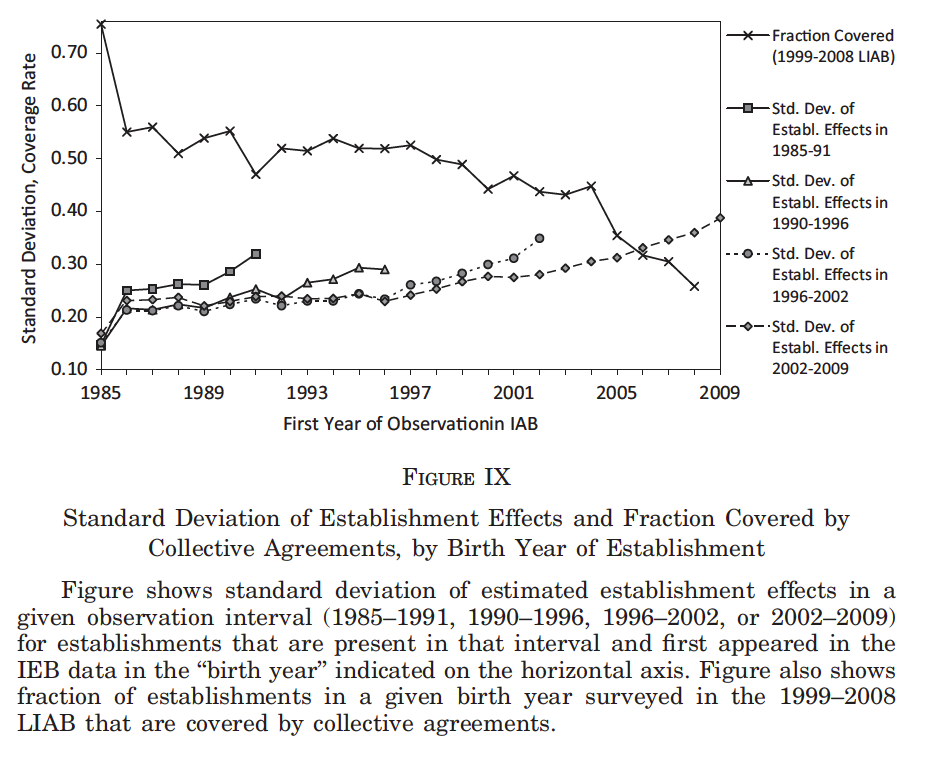
\includegraphics[width=0.9\textwidth]{figures/Fig9} 
\end{figure}
\end{frame}

\begin{frame}{Std. dev. of firm FE increased due to de-unionisation}
\begin{figure}[p!]
 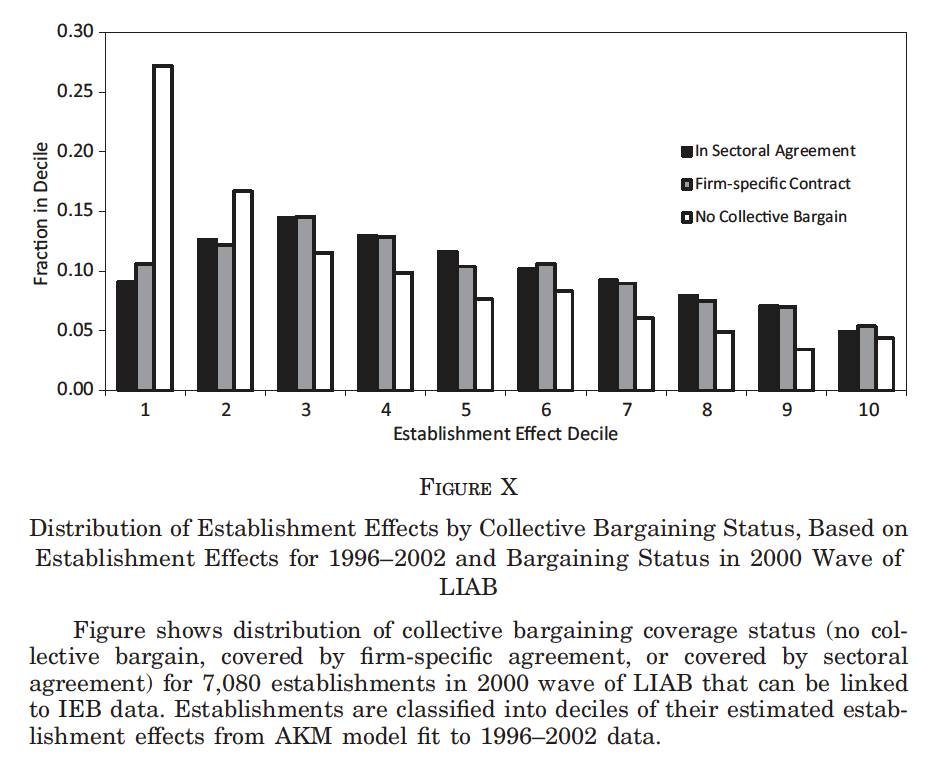
\includegraphics[width=0.9\textwidth]{figures/Fig10} 
\end{figure}
\end{frame}

%%%%%%%%%%%%%%%%%%%%%%%%%%%%%%%%%%%%%%%%%%%%%%%%%%%%%%%%%%%%%%%%%
\section{Conclusion}
%%%%%%%%%%%%%%%%%%%%%%%%%%%%%%%%%%%%%%%%%%%%%%%%%%%%%%%%%%%%%%%%%

\begin{frame}{Conclusion}
\begin{itemize}
	\item This paper studies trends in the dispersion of firm-specific wage premiums and and sorting. \medskip 
	\item Estimate an AKM model using more efficient techniques. \medskip
	\item Rising wage inequality due to rising dispersion in worker- and firm-specific components, and increased sorting. \medskip
    \item Rising dispersion in worker FE explains about 40\%, firm FE 25\%, and increased sorting about 35\% of rising wage inequality in West-Germany between 1985 and 2009. \medskip
    \item This paper has lead to a revival of AKM.
\end{itemize}
\end{frame}

\begin{frame}{Further readings}
\footnotesize
\begin{enumerate}
\item Card, D., Cardoso, A., and Kline, P. (2016). “Bargaining, sorting, and the gender wage gap: quantifying the impact of firms on the relative pay of women”. \textit{Quarterly Journal of Economics}. 131 (2).
\item Goldschmidt, D., and Schmieder, J. (2017). “The rise of domestic outsourcing and the evolution of the German wage structure”. \textit{Quarterly Journal of Economics}. 132 (3).
\item Card, D., Cardoso, A., Heining, J., and Kline, P. (2018). “Firms and labor market inequality: evidence
and some theory”. \textit{Journal of Labor Economics}. 36 (S1).
\item Song, J., Price. D.J., Guvenen, F., Bloom, N., and T. Von Wachter (2019). “Firming up inequality.” \textit{Quarterly Journal of Economics}. 134(1). 
\item Bonhomme, S., Holzeu, K., Lamadon, T., Manresa, E., Mogstad, M., and B. Setzler (2020). “How much should we trust estimates of firm effects and worker sorting?”. \textit{NBER Working Paper} 27368. June 2020. 
\end{enumerate}
\end{frame}

\begin{frame}{Coding}
\begin{itemize}
\item Packages have been written for Stata:
\begin{itemize} \smallskip
    \item \textbf{felsdvreg} \smallskip
    \item \textbf{regxfe} \smallskip
     \item \textbf{a2group} + \textbf{a2reg}
\end{itemize} \smallskip
\item Packages and simulation in R: 
 https://floswald.github.io/ScPo-Labor/lab-akm.html \medskip
\item Card, Heining, and Kline (2013) use matlab - see Pat Kline's webpage for code. \medskip
\item Bonhomme et al. (2020) use Python - see Magne Mogstad's webpage for code.
\end{itemize}
\end{frame}

\end{document}
